
\chapter{Discussion}
This Chapter presents a overview of the implementation solution, the technical encountered challenges during integration with XNAT and the methods employed to overcome the issues. Several issues emerged throughout development, including data transmission failures, REST API inconsistencies, JSON configuration mismatches.

The initial Problem was that the Container did not appear to receive any input files. To confirm this, a test was realized by adding a script within the Container. The script was designed to write a file named no\_file.txt if no input file was detected at runtime. The successful upload of this no file confirmed that while the container was running, it was not receiving actual input data.

Following the initial diagnosis another test was made. Efforts were made to use the Integration of the REST API within the container to retrieve files, process them, and upload the results.
Despite the API was correctly called, no files results appeared in XNAT. 

Attention shifted to the JSON Command that defines the Container command structure in XNAT. The JSON Command was enhanced to include login credentials and more detailed output specifications. Multiples versions were tested, each with different contexts. Despite these efforts, no successful uploads occurred, and in some cases, the command itself was rejected by XNAT. 

It was conjectured that the Container execution timing could play a role in the failure. To test this, the automation script was modified to introduce a 10-second delay between each container execution. The supposition was that the host system might be under resource pressure when running multiple containers in rapid succession. However, introducing delays did not resolve the core issue: the container still did not receive input files.
%-------------------------------------------------------------------------------------------------------------------------

\section{The Workflow data in XNAT:}

In most of the cases when we press the bottom Run container in XNAT in the manual process, usually the data is automatically provided and the Container handles the data and reload the data back.
But in details when we activate the launching of the Container the platform orchestrates a series of data management and processing steps to facilitate the workflow. At first the system often generates a JSON specification. This specification included the information about the script and the command line, which going to be proceeded,the output place files and the container input, ensuring that the containerized process has access to all relevant instructions. Furthermore after that XNAT identifies the relevant data and prepares it for transfer to the designated computational environment. The data is then mounted or copied to a temporary directory within the host system, ensuring accessibility for the containerized analysis. Once the container is activated, it processes by reading the input data according to the command line script, and develops the output data,lastly the output is written back to the designated result directory on the host. 
Assuming  that the Container has the ability to proceed huge amount of files and also there is a possibility to increase the number of files that can be handled  with the command \texttt{Ulimit}. 
The idea that XNAT mounts or copies the data to a temporary directory within the host system, reveals a important insights into the underlying problem. Copying the data in the host system and mounting her into a volume means that the Container has no access to the Data Bank of XNAT, which can potentially lead to issues related to memory or disk space on the host. This approach may result in resource constraints, This issue can become particularly problematic when large datasets are involved; Although my specific test case involved a relatively small number of files, the container still failed to process the data successfully. This suggests that the problem may not be solely related to dataset size or resource limits.

The Diagram above illustrates the workflow data for a clearer understanding...\\


\begin{figure}
    \centering
    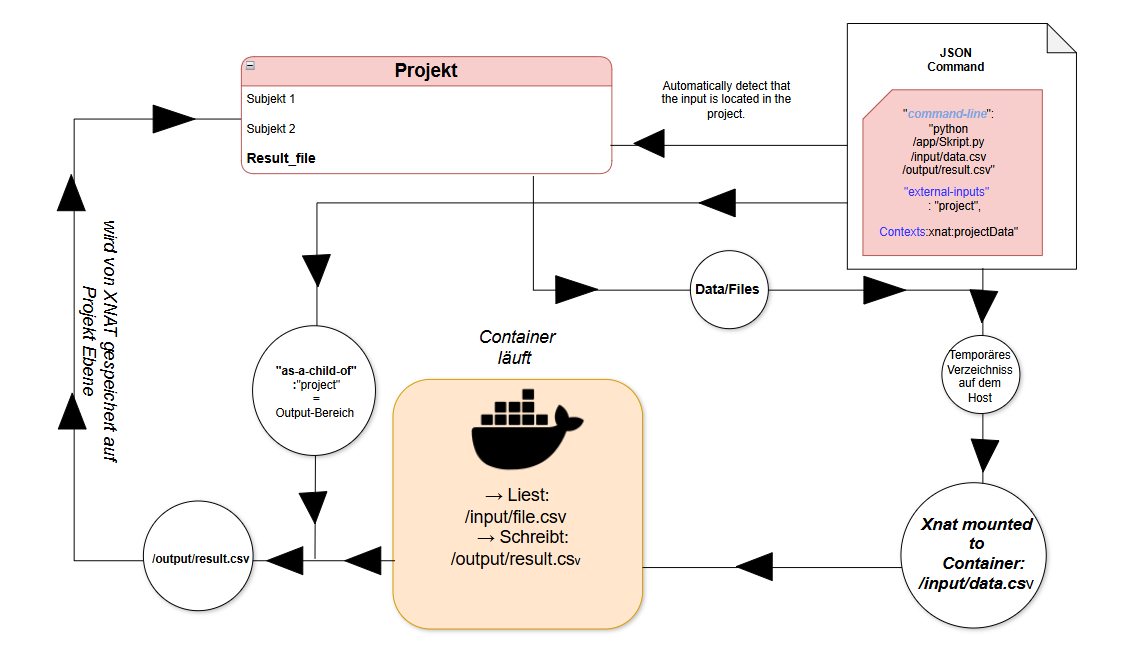
\includegraphics[width=1\linewidth]{en/content/bb.svg}
    \caption{XNAT Workflow Data with the Container  }
    \label{fig:enter-label}
\end{figure}




